\chapter{Warmtestraling}\label{ch:b2:thermal-radiation}

Alles wat warm is, gloeit. Een hand, een muur, een glas water op
kamertemperatuur stralen onzichtbaar, bij golflengten nabij
\qty{10}{\micro m}, enkele honderden watt per vierkante meter; verhit een
pook en bij \qty{600}{\celsius} gloeit hij dofrood, bij
\qty{1000}{\celsius} oranje, bij \qty{2500}{\celsius} --- de gloeidraad
van een lamp --- wit; het oppervlak van de zon straalt bij \qty{5800}{K}
geelwit, zestig megawatt per vierkante meter, en dat licht is, na acht
minuten reizen, wat de aarde op een temperatuur houdt waar water
vloeibaar is. Straling is de derde wijze van warmteoverdracht en de
enige die de lege ruimte oversteekt; zij is ook de plaats waar de
klassieke natuurkunde faalde en Planck in 1900 het kwantum moest
invoeren. Dit hoofdstuk formuleert de wet die hij vond, leidt eruit de
twee uitkomsten af die men voortdurend gebruikt --- de verschuiving van
Wien en de wet van Stefan--Boltzmann --- en past ze toe op de
uitwisselingen tussen lichamen, op de zon en de aarde, en op het
éénlaagsmodel van het \omterm{prop:b2:thermal-radiation:greenhouse}{broeikaseffect} dat ons klimaat bepaalt.

\begin{omfigure}

\includegraphics[width=0.58\linewidth]{images/book4/ai/b4-26-glowing-steel-forge.jpg}

{\small Staal in de smederij: de kleur van de gloed --- dofrood, oranje,
geel, wit --- is een thermometer, omdat het spectrum van \omterm{def:b2:thermal-radiation:blackbody}{warmtestraling}
alleen van de temperatuur afhangt.}
\end{omfigure}

\section{Warmtestraling en het zwarte lichaam}

\begin{definition}[Warmtestraling, absorptievermogen, zwart lichaam]\label{def:b2:thermal-radiation:blackbody}
Elk lichaam op temperatuur $T$ zendt elektromagnetische straling uit door de
warmtebeweging van zijn ladingen: zijn \emph{warmtestraling}\index{warmte
straling}. Zijn oppervlak ontvangt ook
straling uit zijn omgeving en neemt daarvan een deel $\alpha$ op
(het \emph{absorptievermogen}, tussen $0$ en $1$, in het algemeen afhankelijk van
de golflengte), en weerkaatst of laat de rest door. Een \emph{zwart
lichaam}\index{zwart lichaam} neemt alles op ($\alpha = 1$ bij elke
golflengte). Een klein gaatje in de wand van een gesloten holte is het
praktische zwarte lichaam: straling die er binnenkomt wordt aan de wanden opgenomen
voordat zij de weg naar buiten kan vinden.
\end{definition}

\begin{proposition}[Evenwichtsstraling en de wet van Kirchhoff]\label{prop:b2:thermal-radiation:kirchhoff}
Binnen een gesloten holte waarvan de wanden op $T$ staan, is de straling in
evenwicht met de wanden en \emph{universeel}: isotroop,
ongepolariseerd, met een spectrale energiedichtheid $u_\nu(T)$ (energie per
volume-eenheid en per frequentie-eenheid) die alleen van $T$ en $\nu$
afhangt, niet van
het materiaal of de vorm van de holte. De straling die uit een klein gaatje in
zo'n holte vertrekt, is de \emph{zwartlichaamstraling} bij $T$. Een
oppervlak dat het deel $\alpha_\nu$ opneemt van de straling die het ontvangt
bij de frequentie $\nu$, zendt bij die frequentie het deel
$\varepsilon_\nu = \alpha_\nu$ uit van wat een \omterm{def:b2:thermal-radiation:blackbody}{zwart lichaam} bij dezelfde
temperatuur zou uitzenden (zijn \emph{emissievermogen}\index{emissievermogen}):
\emph{goede opnemers zijn goede uitzenders}.
\end{proposition}

\begin{proof}
Universaliteit: verbind twee holten op dezelfde $T$ door een gat met een
filter dat één frequentie doorlaat; als de dichtheden verschilden, zou er energie
van de ene naar de andere stromen bij gelijke temperaturen, in strijd met de tweede
hoofdwet. Kirchhoff: plaats het oppervlak in de holte op zijn eigen $T$; in
evenwicht moet het bij elke frequentie precies uitzenden wat het opneemt,
$\varepsilon_\nu u_\nu = \alpha_\nu u_\nu$.
\end{proof}

\section{De wet van Planck}

\begin{theorem}[Wet van Planck]\label{thm:b2:thermal-radiation:planck}
De spectrale energiedichtheid van zwartlichaamstraling bij de temperatuur
$T$ is
\[
u_\nu(T) = \frac{8\pi h\nu^3}{c^3}\,\frac{1}{\eu^{h\nu/k_BT} - 1},
\]
en het vermogen dat een zwart oppervlak per oppervlakte-eenheid en per
golflengte-eenheid uitstraalt (zijn \emph{spectrale
exitantie}\index{spectrale exitantie}) is
\[
M_\lambda(T) = \frac{2\pi hc^2}{\lambda^5}\,\frac{1}{\eu^{hc/\lambda k_BT} - 1}.
\]
Twee grensgevallen: voor $h\nu \ll k_BT$ is $u_\nu \approx 8\pi\nu^2 k_BT/c^3$
(Rayleigh--Jeans: elke mode van de holte draagt de klassieke energie
$k_BT$ --- een wet die tot oneindig integreert, de ``ultraviolette
catastrofe''); voor $h\nu \gg k_BT$ is
$u_\nu \approx (8\pi h\nu^3/c^3)
\eu^{-h\nu/k_BT}$ (Wien: de boltzmannfactor
van een foton met energie
$h\nu$, \cref{ch:b2:boltzmann-factor}).
\end{theorem}

\begin{proof}
Aangenomen: het tellen van de modes van de holte ($8\pi\nu^2/c^3$ per
volume- en frequentie-eenheid, twee polarisaties) hoort bij het volume van jaar 3,
en de gemiddelde energie van een mode, $h\nu/(\eu^{h\nu/k_BT} - 1)$ in plaats van de
klassieke $k_BT$, is de kwantumhypothese: energie wordt met
de mode in quanta $h\nu$ uitgewisseld, zodat modes met $h\nu \gg k_BT$
bevroren zijn. De betrekking $M_\lambda\,\dd\lambda = (c/4)\,u_\nu\,\dd\nu$ is de
meetkundige factor die in \cref{thm:b2:thermal-radiation:stefan} wordt berekend.
\end{proof}

\begin{omfigure}
\begin{tikzpicture}
  \begin{axis}[omaxis, width=9.2cm, height=5.2cm, xmin=0, xmax=3.1, ymin=0, ymax=1.12,
    xlabel={$\lambda$ (\unit{\micro m})}, ylabel={$M_\lambda$ (wk.)}, xtick={0.5,1,1.5,2,2.5,3}, ytick=\empty, clip=false,
    legend style={font=\scriptsize, at={(0.97,0.95)}, anchor=north east, draw=none, fill=none}]
    \fill[yellow!40, opacity=0.6] (axis cs:0.4,0) rectangle (axis cs:0.7,1.08);
    \addplot[omDef, thick, domain=0.2:3.1, samples=160] {9.25*x^(-5)/(exp(14388/(x*5000))-1)};
    \addlegendentry{\qty{5000}{K}}
    \addplot[omThm, thick, domain=0.25:3.1, samples=160] {9.25*x^(-5)/(exp(14388/(x*4500))-1)};
    \addlegendentry{\qty{4500}{K}}
    \addplot[omExo, thick, domain=0.3:3.1, samples=160] {9.25*x^(-5)/(exp(14388/(x*4000))-1)};
    \addlegendentry{\qty{4000}{K}}
    \node[font=\scriptsize, anchor=south] at (axis cs:0.55,1.08) {zichtbaar};
  \end{axis}
\end{tikzpicture}

{\small Het spectrum van Planck bij drie temperaturen: de piek verschuift naar
kortere golflengten als $1/T$ (Wien) en de oppervlakte groeit als $T^4$
(Stefan). Alleen de heetste kromme legt veel van haar vermogen in de zichtbare
band.}
\end{omfigure}

\begin{omfigure}
\begin{tikzpicture}
  \begin{axis}[omaxis, width=8.6cm, height=4.8cm, xmin=0, xmax=10.9, ymin=0, ymax=2.2,
    xlabel={$x = h\nu/k_BT$}, ylabel={$x^3/(\eu^x - 1)$}, xtick={2,4,6,8,10}, ytick={1,2}, clip=false,
    legend style={font=\scriptsize, at={(0.97,0.95)}, anchor=north east, draw=none, fill=none}]
    \addplot[omDef, thick, domain=0.05:10, samples=160] {x^3/(exp(x)-1)};
    \addlegendentry{Planck}
    \addplot[omExo, thick, dashed, domain=0.05:1.45, samples=60] {x^2};
    \addlegendentry{Rayleigh--Jeans $x^2$}
    \addplot[omThm, thick, dashed, domain=1.2:10, samples=100] {x^3*exp(-x)};
    \addlegendentry{Wien $x^3\eu^{-x}$}
  \end{axis}
\end{tikzpicture}

{\small De functie van Planck en haar twee grensgevallen: klassieke equipartitie
bij lage frequentie, de exponentiële boltzmannafsnijding bij hoge frequentie;
de piek ligt bij $x = 2.82$ (per frequentie-eenheid).}
\end{omfigure}

\begin{proposition}[Verschuivingswet van Wien]\label{prop:b2:thermal-radiation:wien}
De \omterm{thm:b2:thermal-radiation:planck}{spectrale exitantie} $M_\lambda$ piekt bij
\[
\lambda_{\max}\,T = \frac{hc}{4.965\,k_B} = \qty{2.90e-3}{m.K} .
\]
Een lichaam op \qty{300}{K} straalt vooral nabij \qty{10}{\micro m}; de zon
(\qty{5800}{K}) nabij \qty{0.5}{\micro m}, in het groen, waar het oog het
gevoeligst is --- niet toevallig.
\end{proposition}

\begin{proof}
Met $x = hc/\lambda k_BT$ is $M_\lambda \propto x^5/(\eu^x - 1)$; $\dd/\dd x = 0$
geeft $5(\eu^x - 1) = x\eu^x$, dat wil zeggen $x = 5(1 - \eu^{-x})$, waarvan
de wortel
verschillend van nul $x = 4.965$ is.
\end{proof}

\begin{theorem}[Wet van Stefan--Boltzmann]\label{thm:b2:thermal-radiation:stefan}
Een zwart oppervlak op $T$ straalt per oppervlakte-eenheid het totale vermogen
\[
M = \int_0^\infty M_\lambda\,\dd\lambda = \sigma T^4, \qquad
\sigma = \frac{2\pi^5k_B^4}{15h^3c^2} = \qty{5.67e-8}{W/m^2/K^4} ;
\]
de energiedichtheid van de evenwichtsstraling is $u = (4\sigma/c)T^4$
en haar druk $P = u/3$. Een grijs oppervlak met \omterm{prop:b2:thermal-radiation:kirchhoff}{emissievermogen} $\varepsilon$
straalt $\varepsilon\sigma T^4$.
\end{theorem}

\begin{proof}
Integreer de dichtheid van Planck:
$u = \int u_\nu\,\dd\nu = (8\pi h/c^3)(k_BT/h)^4
\int_0^\infty x^3\,\dd x/(\eu^x - 1)$
en de integraal is $\pi^4/15$
(aangenomen uit de analyse): $u = (8\pi^5k_B^4/15h^3c^3)\,T^4$. Het vermogen dat
een gat met eenheidsoppervlak in de holtewand verlaat, is $cu/4$: de
straling is isotroop, de fotonen die naar het gat bewegen binnen de
ruimtehoek $\dd\Omega$ onder de hoek $\theta$ met haar normaal dragen de
flux $c\,u\,(\dd\Omega/4\pi)\cos\theta$, en $\int\cos\theta\,\dd\Omega/4\pi$
over het naar buiten gerichte halfrond is $1/4$. Dus $M = cu/4 = \sigma T^4$.
De druk is, zoals voor elk isotroop gas van deeltjes die met $c$ bewegen,
$u/3$.
\end{proof}

\begin{example}[Ordes van grootte]\label{ex:b2:thermal-radiation:orders}
Bij \qty{300}{K}: $\sigma T^4 = \qty{460}{W/m^2}$ --- een mens van
\qty{1.7}{m^2} straalt \qty{800}{W} uit, maar ontvangt bijna evenveel van
de wanden op \qty{293}{K}; het nettoverlies,
$\sigma A(T^4 - T_0^4) \approx
\qty{100}{W}$, is het volledige
stofwisselingsvermogen van het lichaam, en daarom
heeft men kleren nodig in een kamer die mild aanvoelt. Het zonneoppervlak:
$\sigma
(5800)^4 = \qty{6.4e7}{W/m^2}$, totaal
$3.9 \times 10^{26}\,\unit{W}$. De
gloeidraad van een lamp bij \qty{2800}{K}: \qty{3.5e6}{W/m^2}, \qty{60}{W}
uit een halve
vierkante centimeter wolfraam. De kosmische achtergrond, \qty{2.7}{K}:
piek bij \qty{1}{mm}, $\qty{3e-6}{W/m^2}$, en $400$ fotonen per kubieke
centimeter van het heelal.
\end{example}

\section{Uitwisselingen door straling}

\begin{proposition}[Netto-uitwisseling en de stralingscoëfficiënt]\label{prop:b2:thermal-radiation:exchange}
Een klein grijs lichaam (\omterm{prop:b2:thermal-radiation:kirchhoff}{emissievermogen} $\varepsilon$, oppervlak $S$,
temperatuur $T$)
binnen een grote omgeving op $T_0$ verliest het nettovermogen
\[
P = \varepsilon\sigma S\,(T^4 - T_0^4)
\ \approx\ 4\varepsilon\sigma T_0^3\,S\,(T - T_0) = h_{\text{r}}S(T - T_0)
\quad\text{voor } |T - T_0| \ll T_0 ,
\]
waarin $h_{\text{r}} = 4\varepsilon\sigma T_0^3 \approx \qty{6}{W/m^2/K}$ bij
kamertemperatuur --- vergelijkbaar met natuurlijke convectie: in een kamer
draagt straling ongeveer de helft van de warmte die een lichaam of een
radiator verlaat.
Tussen twee grote evenwijdige zwarte platen is de netto-fluxdichtheid
$\sigma(T_1^4 - T_2^4)$; voor grijze platen met \omterm{prop:b2:thermal-radiation:kirchhoff}{emissievermogens} $\varepsilon_1$,
$\varepsilon_2$ is zij
$\sigma(T_1^4 - T_2^4)/(1/\varepsilon_1 + 1/\varepsilon_2
- 1)$, en elk dun
\emph{stralingsscherm} dat ertussen wordt gezet deelt haar
verder --- het beginsel van de thermosfles en van het goudfolie op
satellieten.
\end{proposition}

\begin{proof}
Het lichaam zendt $\varepsilon\sigma T^4$ uit en neemt het deel
$\alpha =
\varepsilon$ op van de zwarte straling $\sigma T_0^4$ die de
omhulling vult
(Kirchhoff). Lineariseer $T^4 - T_0^4 \approx 4T_0^3(T - T_0)$. Voor de
grijze platen telt men de veelvuldige weerkaatsingen op (een meetkundige reeks).
\end{proof}

\begin{example}[Vorst onder een heldere hemel, en de warmtebeeldcamera]\label{ex:b2:thermal-radiation:frost}
In een heldere nacht straalt de hemel als een lichaam op ongeveer \qty{250}{K}
(de droge hogere dampkring), terwijl de lucht bij de grond op
\qty{278}{K} staat. Een blad of een autodak ($\varepsilon = 0.95$) brengt zijn
stralingsverlies naar de hemel in evenwicht met convectie van de lucht
($h =
\qty{5}{W/m^2/K}$): $\varepsilon\sigma(T^4 - 250^4) = h(278 - T)$
geeft $T
\approx \qty{266}{K}$ --- vorst bij \qty{-7}{\celsius} op het gras
terwijl
de thermometer $+5$ aanwijst. Een wolk (die bij \qty{275}{K} straalt) tilt $T$
naar \qty{277}{K}: geen vorst. Een warmtebeeldcamera meet de
stralingsdichtheid nabij
\qty{10}{\micro m} en zet die om in een temperatuur in de veronderstelling
$\varepsilon \approx 0.95$; een gepolijst metaal ($\varepsilon = 0.1$) weerkaatst
vooral de kamer en lijkt op de temperatuur van de kamer te staan, wat de
zijne ook is
--- vandaar de zwarte tape die thermografen op glimmende delen plakken.
\end{example}

\section{De zon, de aarde en de broeikas}

\begin{proposition}[Zonneconstante en effectieve temperatuur]\label{prop:b2:thermal-radiation:earth}
De zon (straal $R_\odot$, oppervlaktetemperatuur $T_\odot$) levert op de
afstand $d$ de fluxdichtheid
$S = \sigma T_\odot^4 (R_\odot/d)^2 =
\qty{1361}{W/m^2}$ boven de dampkring
van de aarde (de \emph{zonneconstante}\index{zonne
constante}). Een planeet met albedo $A$ (het weerkaatste
deel) neemt $(1 - A)S\pi R^2$ op en straalt dat in de stationaire toestand
van haar hele oppervlak $4\pi R^2$ uit als een \omterm{def:b2:thermal-radiation:blackbody}{zwart lichaam} op haar
\emph{effectieve
temperatuur}\index{effectieve temperatuur}
\[
T_{\text{e}} = \Big(\frac{(1 - A)S}{4\sigma}\Big)^{1/4} = \qty{255}{K}
\quad\text{voor de aarde } (A = 0.30) .
\]
\end{proposition}

\begin{proof}
Energiebehoud: opgenomen $= $ uitgezonden, de doorsnede $\pi R^2$
voor de onderschepte bundel, de volle bol voor de uitzending (dag en
nacht, gespreid door draaiing en circulatie).
\end{proof}

\begin{omfigure}
\begin{tikzpicture}[scale=0.95, >=stealth]
  % ground
  \fill[omExo!15] (0,0) rectangle (8,0.6);
  \draw[thick] (0,0.6) -- (8,0.6);
  \node[font=\scriptsize] at (4,0.3) {oppervlak $T_{\text{s}}$};
  % atmosphere layer
  \fill[omDef!12] (0,2.6) rectangle (8,3.0);
  \draw (0,2.6) -- (8,2.6); \draw (0,3.0) -- (8,3.0);
  \node[font=\scriptsize] at (4.3,2.8) {dampkring $T_{\text{a}}$};
  % solar in
  \draw[->, yellow!60!orange, very thick] (1.2,4.3) -- (1.2,0.7);
  \node[font=\scriptsize, yellow!50!orange, left] at (1.1,3.8) {$(1 - A)S/4$};
  % surface up
  \draw[->, omThm, very thick] (3.2,0.7) -- (3.2,2.5);
  \node[font=\scriptsize, omThm, right] at (3.25,1.6) {$\sigma T_{\text{s}}^4$};
  % atm up & down
  \draw[->, omDef, very thick] (5.4,3.1) -- (5.4,4.3);
  \node[font=\scriptsize, omDef, right] at (5.45,3.8) {$\sigma T_{\text{a}}^4$};
  \draw[->, omDef, very thick] (6.8,2.5) -- (6.8,0.7);
  \node[font=\scriptsize, omDef, right] at (6.85,1.6) {$\sigma T_{\text{a}}^4$};
  \node[font=\scriptsize] at (4,4.6) {ruimte};
\end{tikzpicture}

{\small De broeikas met één laag: zonlicht doorkruist de dampkring en
verwarmt de grond; het infrarood van de grond wordt door de laag opgenomen, die
half omhoog en half omlaag straalt --- het oppervlak moet dan twee keer
uitstralen wat het van de zon ontvangt.}
\end{omfigure}

\begin{proposition}[Broeikasmodel met één laag]\label{prop:b2:thermal-radiation:greenhouse}
Omgeef de planeet met een dunne laag dampkring die doorzichtig is
voor zonlicht maar al het infrarood opneemt dat het oppervlak uitzendt, en
die als een \omterm{def:b2:thermal-radiation:blackbody}{zwart lichaam} op $T_{\text{a}}$ zowel omhoog als omlaag straalt. In de
stationaire toestand geldt
\[
T_{\text{a}} = T_{\text{e}}, \qquad
T_{\text{s}} = 2^{1/4}\,T_{\text{e}} = \qty{303}{K} .
\]
Als de laag maar het deel $\varepsilon$ van het infrarood opneemt, is
$T_{\text{s}}^4 = T_{\text{e}}^4/(1 - \varepsilon/2)$; de waargenomen
\qty{288}{K} komt overeen met $\varepsilon \approx 0.78$. Het oppervlak is
warmer dan de \omterm{prop:b2:thermal-radiation:earth}{effectieve temperatuur} omdat het, naast
de zon, het infrarood ontvangt dat de dampkring terugstuurt --- het
\emph{broeikaseffect}\index{broeikaseffect}, \qty{33}{K} op aarde,
zonder hetwelk de oceanen bevroren zouden zijn.
\end{proposition}

\begin{proof}
Balans van de laag: neemt $\sigma T_{\text{s}}^4$ op, zendt
$2\sigma
T_{\text{a}}^4$ uit. Balans van de planeet vanuit de ruimte gezien:
zendt $\sigma
T_{\text{a}}^4 = (1 - A)S/4 = \sigma T_{\text{e}}^4$ uit.
Balans van het
oppervlak: ontvangt $(1 - A)S/4 + \sigma T_{\text{a}}^4 = 2\sigma T_{\text{e}}^4$,
zendt $\sigma T_{\text{s}}^4$ uit. Vervang voor de gedeeltelijke laag het
opgenomen en uitgezonden infrarood door $\varepsilon\sigma T_{\text{s}}^4$ en
$\varepsilon\sigma T_{\text{a}}^4$ en laat het deel $1 - \varepsilon$
van de oppervlaktestraling rechtstreeks ontsnappen.
\end{proof}

\begin{omfigure}
\begin{tikzpicture}
  \begin{axis}[width=9.6cm, height=5cm, xmode=log, xmin=0.1, xmax=100, ymin=0, ymax=1.15,
    axis x line=bottom, axis y line=left, xlabel={$\lambda$ (\unit{\micro
    m})}, ylabel={$M_\lambda$ (genormeerd)},
    xlabel style={at={(axis description cs:0.5,-0.12)}, anchor=north},
    xtick={0.1,1,10,100}, xticklabels={$0.1$,$1$,$10$,$100$}, ytick=\empty, clip=false,
    legend style={font=\scriptsize, at={(0.02,0.97)}, anchor=north west, draw=none, fill=none}]
    \fill[omDef!10] (axis cs:5,0) rectangle (axis cs:8,1.0);
    \fill[omDef!10] (axis cs:14,0) rectangle (axis cs:17,1.0);
    \fill[gray!10] (axis cs:2.6,0) rectangle (axis cs:2.9,1.0);
    \addplot[yellow!60!orange, thick, domain=0.1:8, samples=200] {4.4*x^(-5)/(exp(14388/(x*5800))-1)};
    \addlegendentry{zon, \qty{5800}{K}}
    \addplot[omExo, thick, domain=2.5:100, samples=200] {1.41e7*x^(-5)/(exp(14388/(x*288))-1)};
    \addlegendentry{aarde, \qty{288}{K}}
    \node[font=\tiny, omDef, anchor=south] at (axis cs:6.3,1.0) {H$_2$O};
    \node[font=\tiny, omDef, anchor=south] at (axis cs:15.5,1.0) {CO$_2$};
    \node[font=\tiny, anchor=south] at (axis cs:10.5,0.2) {venster};
  \end{axis}
\end{tikzpicture}

{\small De spectra van de zon en de aarde (elk op zijn eigen piek
genormeerd) overlappen nauwelijks: de dampkring kan doorzichtig zijn voor het ene en
ondoorzichtig voor het andere. Gearceerd: de belangrijkste
infraroodabsorptiebanden van
waterdamp en koolstofdioxide; daartussen het venster van
\qty{8}{}--\qty{13}{\micro m}
waardoor het oppervlak rechtstreeks naar de ruimte straalt.}
\end{omfigure}

\begin{remark}[Waarom de broeikas selectief is]\label{rem:b2:thermal-radiation:selective}
Zonlicht piekt bij \qty{0.5}{\micro m}, de straling van de aarde bij
\qty{10}{\micro m}: de twee spectra overlappen nauwelijks, zodat een gas
doorzichtig kan zijn voor het eerste en absorberend voor het tweede. Stikstof en
zuurstof nemen geen van beide op; waterdamp, koolstofdioxide, methaan en ozon
hebben trillingsbanden in het infrarood en zijn de broeikasgassen. Het
venster tussen \qty{8}{} en \qty{13}{\micro m} is waar de warmtebeeldcamera
doorheen kijkt, waar de \qty{250}{K} van de nachthemel op slaat, en wat
verven voor stralingskoeling benutten. Het glas van een echte kas doet
hetzelfde (doorzichtig bij \qty{0.5}{\micro m}, ondoorzichtig bij
\qty{10}{\micro m}),
maar vooral houdt het convectie tegen --- de naam is een beetje onbillijk.
\end{remark}

\begin{method}[Stralingsschattingen]\label{meth:b2:thermal-radiation:method}
(1) $\lambda_{\max} = \qty{2900}{\micro m.K}/T$ zegt waar het spectrum
ligt; (2) $\varepsilon\sigma T^4$ per oppervlakte-eenheid; (3)
uitwisselingen: uitgezonden
min opgenomen, gelineariseerd als $h_{\text{r}} = 4\varepsilon\sigma T^3$ nabij
kamertemperatuur; (4) een planeet: $(1 - A)S/4 = \sigma T_{\text{e}}^4$, dan
de lagen; (5) vergelijk met geleiding en convectie --- straling
wint bij hoge temperatuur ($T^4$) en in vacuüm; (6) let op \omterm{prop:b2:thermal-radiation:kirchhoff}{emissievermogens}:
glimmende metalen \qty{0.05}{}, verven, huid, water, bodem $\approx 0.9$--$0.98$
in het infrarood, welke zichtbare kleur zij ook hebben.
\end{method}

\section{Opgaven}

\begin{exercise}[$\star$]\label{exo:b2:thermal-radiation:1}
$\lambda_{\max}$ en $\sigma T^4$ voor: de zon (\qty{5800}{K}), een mens
(\qty{310}{K}), de gloeidraad van een lamp (\qty{2800}{K}), de kosmische achtergrond
(\qty{2.73}{K}), vloeibare stikstof (\qty{77}{K}), een roodgloeiende pook
(\qty{900}{K}). Welke zijn zichtbaar?
\end{exercise}

\begin{exercise}[$\star$]\label{exo:b2:thermal-radiation:2}
Uit $T_\odot = \qty{5772}{K}$, $R_\odot = \qty{6.96e8}{m}$, $d = \qty{1.496e11}{m}$:
de \omterm{prop:b2:thermal-radiation:earth}{zonneconstante}, de lichtkracht van de zon, het vermogen dat de aarde
onderschept ($R = \qty{6.37e6}{m}$), en hetzelfde verdeeld over $8 \times 10^9$
mensen. Vergelijk met het wereldwijde vermogensverbruik (\qty{2e13}{W}).
\end{exercise}

\begin{exercise}[$\star$]\label{exo:b2:thermal-radiation:3}
Een mens: huid op \qty{306}{K}, $\varepsilon = 0.98$, \qty{1.7}{m^2}, in een
kamer op \qty{293}{K}. Uitgezonden vermogen, opgenomen vermogen, nettoverlies; de
stralingscoëfficiënt $h_{\text{r}}$; vergelijk met de \qty{100}{W} van de
stofwisseling en besluit over kleren en over een kamer van \qty{20}{\celsius}
met koude wanden.
\end{exercise}

\begin{exercise}[$\star$]\label{exo:b2:thermal-radiation:4}
Een lamp van \qty{60}{W}: wolfraamdraad op \qty{2800}{K}, $\varepsilon = 0.35$.
Stralend oppervlak; lengte van een draad van \qty{50}{\micro m} met dat oppervlak;
ongeveer $8\%$ van het vermogen is zichtbaar: lichtvermogen; een led die
hetzelfde licht geeft bij $30\%$ rendement.
\end{exercise}

\begin{exercise}[$\star\star$]\label{exo:b2:thermal-radiation:5}
\emph{De twee grensgevallen.} (a) Ontwikkel de $u_\nu$ van Planck voor
$h\nu \ll k_BT$ en
wijs de energie per mode aan. (b) Toon aan dat de wet van Rayleigh--Jeans
een oneindige totale energie geeft. (c) Bij \qty{300}{K}, de frequentie waar
$h\nu = k_BT$; besluit dat \omterm{def:b2:thermal-radiation:blackbody}{warmtestraling} in radio- en microgolven
klassiek is. (d) Duid $\eu^{-h\nu/k_BT}$ in het grensgeval van Wien.
\end{exercise}

\begin{exercise}[$\star\star$]\label{exo:b2:thermal-radiation:6}
\emph{Wien.} (a) Leid $x = 5(1 - \eu^{-x})$ af en los het getalsmatig
op tot drie cijfers. (b) Waarde van $\lambda_{\max}T$. (c) Toon aan dat $u_\nu$
piekt bij $h\nu = 2.82\,k_BT$, en dat dit niet overeenkomt met
$c/\lambda_{\max}$: waarom niet? (d) Temperatuur van een ster waarvan het spectrum
bij \qty{290}{nm} piekt; haar kleur voor het oog.
\end{exercise}

\begin{exercise}[$\star\star$]\label{exo:b2:thermal-radiation:7}
\emph{Stefan.} (a) Voer de integratie van de wet van Planck uit, gegeven
$\int_0^\infty x^3\dd x/(\eu^x - 1) = \pi^4/15$, en de waarde van $\sigma$.
(b) Verantwoord de factor $c/4$ tussen de dichtheid en de exitantie. (c)
Gegeven $\int_0^\infty x^2\dd x/(\eu^x - 1) = 2.404$, het aantal fotonen
per volume-eenheid bij $T$, en de gemiddelde fotonenergie in eenheden van $k_BT$.
(d) Fotonen per kubieke centimeter bij \qty{300}{K} en bij \qty{2.73}{K}.
\end{exercise}

\begin{exercise}[$\star\star$]\label{exo:b2:thermal-radiation:8}
\emph{Schermen.} Twee grote zwarte platen op $T_1$, $T_2$. (a) Nettoflux.
(b) Er wordt een dun zwart blad tussen gezet: zijn temperatuur en de
nieuwe flux. (c) $n$ bladen. (d) Grijze platen met \omterm{prop:b2:thermal-radiation:kirchhoff}{emissievermogen} $\varepsilon$:
toon aan dat de flux $\sigma(T_1^4 - T_2^4)/(2/\varepsilon - 1)$ is en bereken
haar voor gepolijste oppervlakken ($\varepsilon = 0.05$) bij \qty{300}{K} en
\qty{77}{K} --- de thermosfles.
\end{exercise}

\begin{exercise}[$\star\star$]\label{exo:b2:thermal-radiation:9}
\emph{Nachtvorst.} Oppervlak $\varepsilon = 0.95$, hemel op \qty{250}{K}, lucht op
\qty{278}{K} met $h = \qty{5}{W/m^2/K}$. (a) Schrijf de balans en los haar op
voor de oppervlaktetemperatuur. (b) Onder een wolk op \qty{275}{K}. (c) Waarom
belet wind vorst? (d) Waarom ontsnapt een auto die onder een boom staat eraan?
\end{exercise}

\begin{exercise}[$\star\star\star$]\label{exo:b2:thermal-radiation:10}
\emph{Planeten.} (a) Effectieve temperaturen van Venus ($S = \qty{2600}{W/m^2}$,
$A = 0.75$), de aarde, Mars ($S = \qty{590}{W/m^2}$, $A = 0.25$). (b) Hun
oppervlaktetemperaturen zijn \qty{737}{K}, \qty{288}{K}, \qty{215}{K}:
broeikasopwarming van elk. (c) Toon in het model met $n$ ondoorzichtige lagen
aan dat $T_{\text{s}}^4 = (n + 1)T_{\text{e}}^4$; hoeveel lagen voor Venus?
(d) De maan: $A = 0.12$, geen dampkring, trage draaiing --- temperatuur
van het subsolaire punt, en waarom de nachtzijde tot \qty{100}{K} zakt.
\end{exercise}

\begin{exercise}[$\star\star\star$]\label{exo:b2:thermal-radiation:11}
\emph{Klimaatgevoeligheid zonder \omterm{def:b2:feedback-oscillators:loop}{terugkoppelingen}.} (a) Lineariseer de
planetaire balans: een kleine extra forcering $\Delta F$ (in \unit{W/m^2}) aan
de bovenkant van de dampkring verhoogt de \omterm{prop:b2:thermal-radiation:earth}{effectieve temperatuur} met
$\Delta T
= \Delta F/4\sigma T_{\text{e}}^3$. Bereken
$4\sigma T_{\text{e}}^3$. (b)
Het verdubbelen van de koolstofdioxide is een forcering van ongeveer
\qty{3.7}{W/m^2}:
$\Delta T$ in dit model. (c) De gemengde laag van de oceaan (\qty{50}{m}
water) slaat de warmte op: tijdconstante van het antwoord. (d) Waarom maken de
\omterm{def:b2:feedback-oscillators:loop}{terugkoppelingen} van waterdamp en ijsalbedo de werkelijke gevoeligheid groter
dan (b)?
\end{exercise}

\begin{exercise}[$\star\star\star$]\label{exo:b2:thermal-radiation:12}
\emph{Pyrometrie.} (a) Toon in het grensgeval van Wien aan dat de verhouding van de
stralingsdichtheden bij twee golflengten, $\lambda_1$ en $\lambda_2$, $T$ geeft
onafhankelijk van een grijs \omterm{prop:b2:thermal-radiation:kirchhoff}{emissievermogen}. (b) Een stalen staaf:
$M_{0.65}/M_{0.9}
= 0.10$: temperatuur. (c) Een warmtebeeldcamera bij
\qty{10}{\micro m} veronderstelt
$\varepsilon = 0.95$; zij kijkt naar gepolijst aluminium ($\varepsilon = 0.1$)
op \qty{350}{K} in een kamer op \qty{293}{K}: welke temperatuur meldt zij
in het gelineariseerde regime? (d) Waarom leest een geverfd oppervlak naast
het aluminium, op dezelfde \qty{350}{K}, wel juist af?
\end{exercise}

\begin{omfigure}
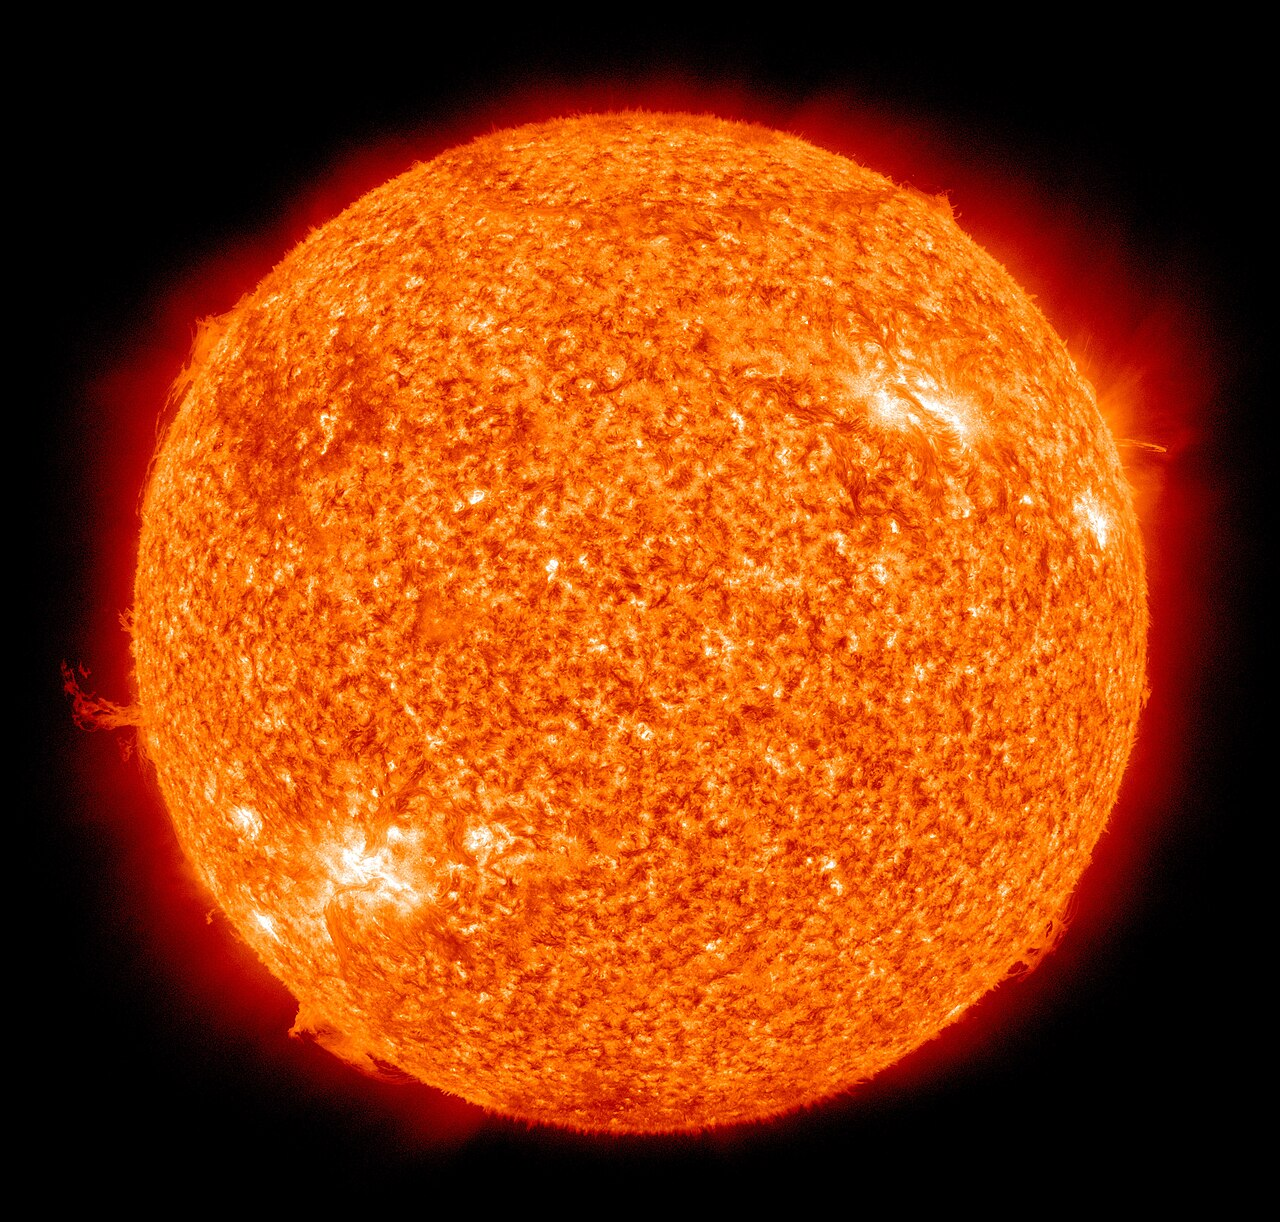
\includegraphics[width=0.4\linewidth]{images/book4/sun-sdo-aia.jpg}\hfill
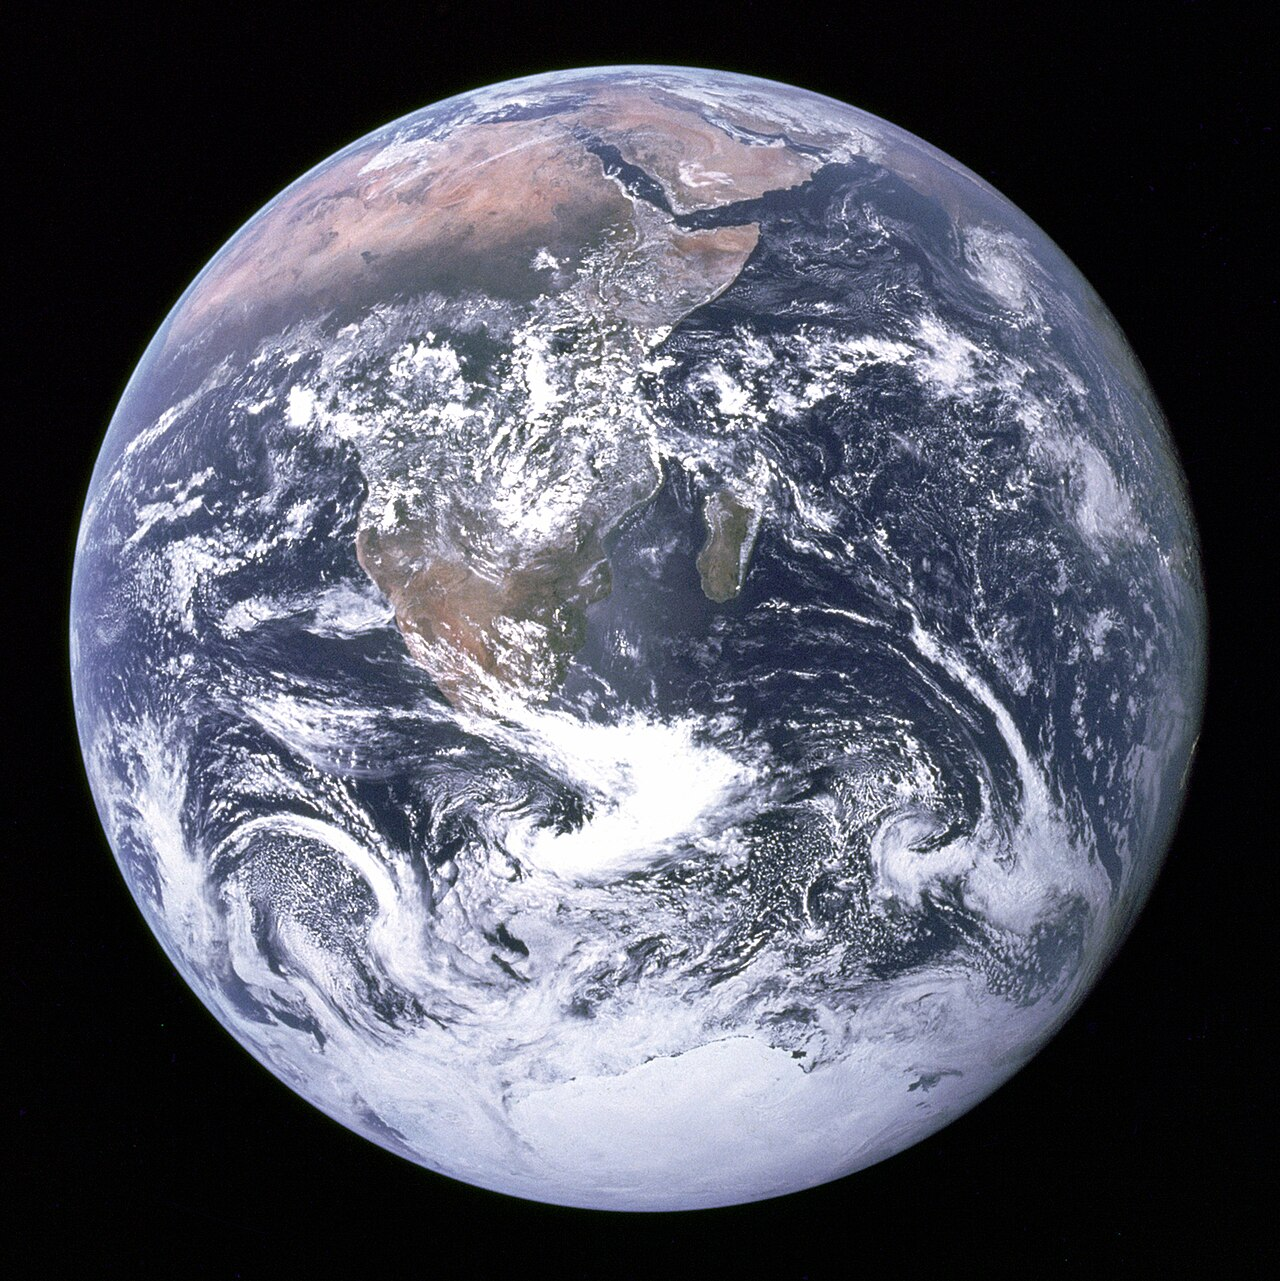
\includegraphics[width=0.4\linewidth]{images/book4/earth-apollo17.jpg}

{\small De twee zwarte lichamen van dit hoofdstuk: de zon, bij
\qty{5800}{K}, gezien door het Solar Dynamics Observatory in het extreme
ultraviolet, en de aarde, bij \qty{288}{K}, gefotografeerd door de bemanning
van Apollo 17 --- pieken bij \qty{0.5}{\micro m} en bij \qty{10}{\micro m}
(NASA).}
\end{omfigure}

\section{Vraagstuk: de energiebalans van de aarde en de gloeilamp}

\begin{problem}[{Weekendvraagstuk --- zwarte lichamen van de zon tot de
gloeidraad}]\label{pb:b2:thermal-radiation:1}
Gegevens: $\sigma = \qty{5.67e-8}{W/m^2/K^4}$,
$\lambda_{\max}T = \qty{2.90e-3}{m.K}$,
$h = \qty{6.63e-34}{J.s}$, $k_B = \qty{1.38e-23}{J/K}$, $c = \qty{3.00e8}{m/s}$;
zon: $R_\odot = \qty{6.96e8}{m}$, $d = \qty{1.50e11}{m}$; aarde:
$R =
\qty{6.37e6}{m}$, albedo $0.30$.

\textbf{Deel I --- De zon als \omterm{def:b2:thermal-radiation:blackbody}{zwart lichaam}.}
\begin{enumerate}
  \item Het zonnespectrum piekt bij \qty{0.50}{\micro m}: oppervlakte\-temperatuur.
  \item Exitantie van het oppervlak en totale lichtkracht.
  \item \omterm{prop:b2:thermal-radiation:earth}{Zonneconstante} bij de aarde; energiedichtheid en druk van
        het zonlicht daar.
  \item Gemiddelde fotonenergie ($\approx 2.7\,k_BT$) en aantal zonnefotonen
        per seconde en per vierkante meter bij de aarde.
  \item De zon straalt al $4.5 \times 10^9$ jaar met dit tempo:
        uitgezonden energie; vergelijk met $Mc^2$ voor $M = \qty{2e30}{kg}$.
\end{enumerate}

\textbf{Deel II --- De aarde zonder dampkring.}
\begin{enumerate}[resume]
  \item Vermogen dat de aarde opneemt; \omterm{prop:b2:thermal-radiation:earth}{effectieve temperatuur}.
  \item Waarom deelt de balans door $4$? Wat zou de
        temperatuur zijn in het subsolaire punt van een niet-draaiende aarde zonder
        dampkring ($A = 0.30$)?
  \item De maan ($A = 0.12$): subsolaire temperatuur; en waarom haar nachtzijde
        tot \qty{100}{K} zakt (denk aan de warmte die tijdens de dag van
        twee weken in het regoliet wordt opgeslagen, werkzaam \qty{1e6}{J/m^2/K}).
  \item Golflengte van de emissiepiek van de aarde; vergelijk met die
        van de zon.
  \item Als meer ijs of wolken het albedo tot $0.35$ verhoogden, met hoeveel
        zou de \omterm{prop:b2:thermal-radiation:earth}{effectieve temperatuur} dalen?
\end{enumerate}

\textbf{Deel III --- De broeikas.}
\begin{enumerate}[resume]
  \item Schrijf de drie balansen (ruimte, laag, oppervlak) van het
        éénlaagsmodel op en verkrijg $T_{\text{s}} = 2^{1/4}T_{\text{e}}$.
  \item Met een laag die het deel $\varepsilon$ van het infrarood opneemt:
        $T_{\text{s}}(\varepsilon)$; de waarde van $\varepsilon$
        die \qty{288}{K} geeft.
  \item Welke gassen nemen op, welke niet, en in welke golflengteband;
        wat is het atmosferische venster?
  \item Het infrarood dat de dampkring naar de grond terugstuurt,
        in \unit{W/m^2}, in het model met $\varepsilon = 0.78$; vergelijk met
        het opgenomen zonlicht.
  \item Een forcering van \qty{3.7}{W/m^2} (verdubbelde koolstofdioxide):
        temperatuurverandering $\Delta T = \Delta F/4\sigma T_{\text{e}}^3$
        zonder \omterm{def:b2:feedback-oscillators:loop}{terugkoppelingen}.
  \item Warmtecapaciteit van een gemengde oceaanlaag van \qty{50}{m} per vierkante
        meter en de tijdconstante van het antwoord.
  \item Waarom koelen wolken het oppervlak (albedo) én verwarmen zij het
        (infrarood); welk effect wint 's nachts?
\end{enumerate}

\textbf{Deel IV --- De gloeilamp.}
Een lamp van \qty{60}{W} heeft een wolfraamdraad op \qty{2800}{K},
$\varepsilon = 0.35$; het deel van het vermogen van een \omterm{def:b2:thermal-radiation:blackbody}{zwart lichaam} dat in
het zichtbare valt ($0.4$--\qty{0.7}{\micro m}) is $0.08$ bij \qty{2800}{K}
en $0.14$
bij \qty{3200}{K}.
\begin{enumerate}[resume]
  \item Stralend oppervlak van de gloeidraad; lengte van een draad van
        \qty{50}{\micro m}
        die het heeft; waarom is hij opgerold?
  \item Piekgolflengte; zichtbaar vermogen; lichtrendement.
  \item Weerstand van de gloeidraad in bedrijf bij \qty{230}{V};
        de \omterm{prop:b2:charges-currents-conduction:drude}{soortelijke weerstand} van wolfraam is bij kamertemperatuur
        ongeveer tien keer kleiner:
        stroom bij het inschakelen, en een gevolg daarvan.
  \item Bij \qty{3200}{K}: het oppervlak dat voor dezelfde \qty{60}{W} nodig is en
        het zichtbare vermogen; waarom niet elke lamp op \qty{3200}{K} laten lopen
        (het verdampingstempo van het wolfraam verdubbelt ruwweg om de
        \qty{50}{K})?
  \item Wat doet de halogeenkringloop, en waarom laat zij een hetere
        gloeidraad toe?
  \item Waar gaat de rest van de \qty{60}{W} heen, en waarom bereikt het glas
        van de lamp \qty{150}{\celsius}?
  \item De afkoeltijd van de gloeidraad na het uitschakelen: schat die uit
        zijn massa (\qty{20}{mg}, $c = \qty{140}{J/kg/K}$) en zijn uitgestraalde
        vermogen.
  \item Vat samen: wat de temperatuur van een \omterm{def:b2:thermal-radiation:blackbody}{zwart lichaam} vastlegt, en wat
        de gloeidraad, de zon en de aarde gemeen hebben.
\end{enumerate}
\end{problem}
